In order to test the validity of using neural networks sampled
from molecular dynamics trajectories to generate new trajectories
we train neural networks on systems of copper and silicon atoms
using the Effective Medium Theory and Stillinger-Weber potentials
respectively. These potentials have efficient implementations
through ASE and their ASAP interface, which makes
it ideal for our purposes. Additionally these potentials
have an intermediate complexity, with Stillinger-Weber explicitly
including threebody interactions, which makes them ideal
for testing whether the Behler-Parrinello method can replicate this.
At temperatures which are not too large these potentials describe
atoms in a crystalline structure in equilibrium,
and we test whether the neural network can reproduce the correct potential
energy, forces, radial distribution and mean squared displacement.
In table \ref{tab:hyperparam} we have listed the parameters we have
used in the training process. While we have used a large amount
of training images for the energy training, since this is relatively
inexpensive, 20000 training images was a noticeable over approximately
5000-10000 images, and only seemed to affect the speed of convergence.
In table \ref{tab:hyperparam-test} we have listed the parameters
used for testing the neural network. For sampling data we used a larger
timestep and sampling interval
than for applying the neural network, in order to obtain
a larger diversity of configurations, though this did not seem to
matter much for the final result.

\begin{table}[H]
\centering
\begin{tabular}{|c c|}
\hline
Hyperparameter & Value \\
\hline \hline
Symmetry functions & 16 radial, 24 angular \\
    Hidden layers & $(10, 10)$ \\
Activation & Hyperbolic tangent \\
    Time (fs) & $2 \cdot 10^6$ \\
    Timestep (fs) & 5 \\
    Sampling intervall (fs) & 100 \\
Max epochs & 4000 \\
Optimizer & BFGS \\
Energy coefficient & 1.0 \\
Force coefficient & 0.1 \\
\hline
\end{tabular}
\caption{Hyperparameters used in fitting.}
\label{tab:hyperparam}
\end{table}

\begin{table}[H]
\centering
\begin{tabular}{|c c|}
\hline
Hyperparameter & Value \\
\hline \hline
Symmetry functions & 16 radial, 24 angular \\
    Hidden layers & $(10, 10)$ \\
Activation & Hyperbolic tangent \\
    Time (fs) & $5 \cdot 10^3$ \\
    Timestep (fs) & 1 \\
    Sampling intervall (fs) & 10 \\
\hline
\end{tabular}
\caption{Hyperparameters used in testing.}
\label{tab:hyperparam-test}
\end{table}

\subsection{Effective Medium Theory}
The Effective Medium Theory (EMT) potential gives a good description
of the late transition metals in a Face-Centered Cubic (FCC) crystal
lattice, and has a very efficient implementation in ASE,
which makes it ideal for producing large amounts of data.
We will use a rather small system of $4 \times 2^3 = 32$ atoms
for training, since this means a larger amount of labels available
for atoms when we are only using the potential energy.
We train with only the energy for $8 \cdot 10^5$ steps
with a timestep of $\Delta t = 5.0$ fs
writing to file every 100 steps and then subsequently
train using both energy and forces for $5 \cdot 10^4$ steps
for a total of 500 configurations. We train on both sets of images
for 2000 steps, where the BFGS optimizer has generally converged.
After the calculator is trained we compare the performance
of the neural network with the EMT potential on a system
of 32 atoms with a temperature of 300 Kelvin for 5000 steps.

\begin{figure}[H]
\begin{adjustbox}{max width=1.2\linewidth,center}
\centering
  \begin{subfigure}[b]{0.55\textwidth}
      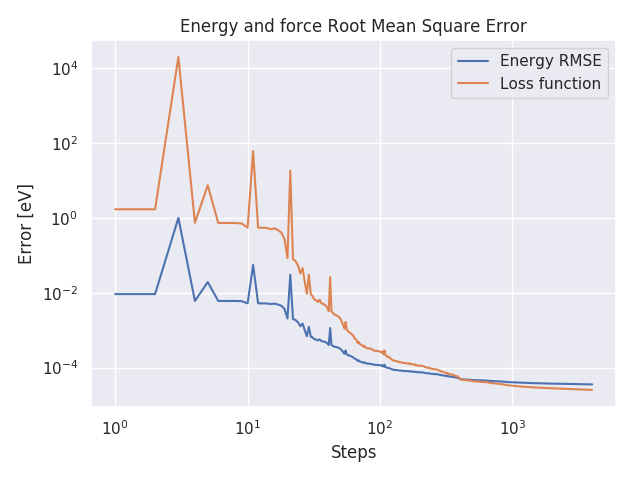
\includegraphics[width=\textwidth]{copper_energy_log.png}
      \caption{Training loss and energy RMSE.}
    \label{fig:f1}
  \end{subfigure}
  \hfill
  \begin{subfigure}[b]{0.55\textwidth}
      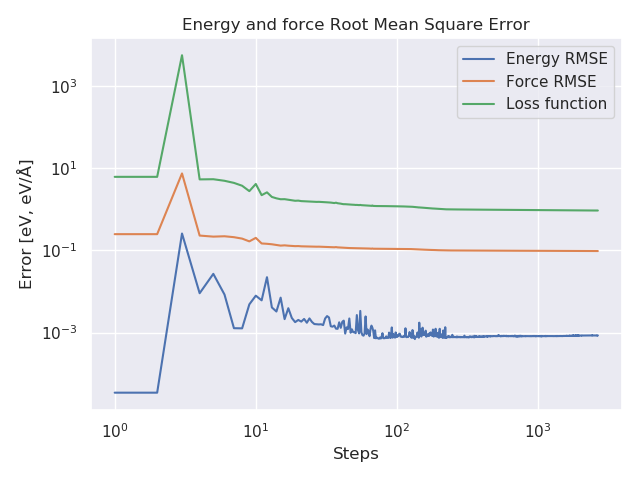
\includegraphics[width=\textwidth]{copper_force_log.png}
      \caption{Training loss and energy and force RMSE.}
    \label{fig:f2}
  \end{subfigure}
\end{adjustbox}
\caption{My flowers.}
    \label{fig:copper_log}
\end{figure}

In figure \ref{fig:copper_log} we have plotted the loss and root mean
squared errors for the training process.
We see that the training process for the energy training
continues to decrease after about 1000 steps, though
the updates are smaller than before.
For the force training we have converged after
approximately 200-400 steps, after which the energy RMSE
stabilizes.

\begin{figure}[H]
\begin{adjustbox}{max width=1.2\linewidth,center}
\centering
  \begin{subfigure}[b]{0.55\textwidth}
      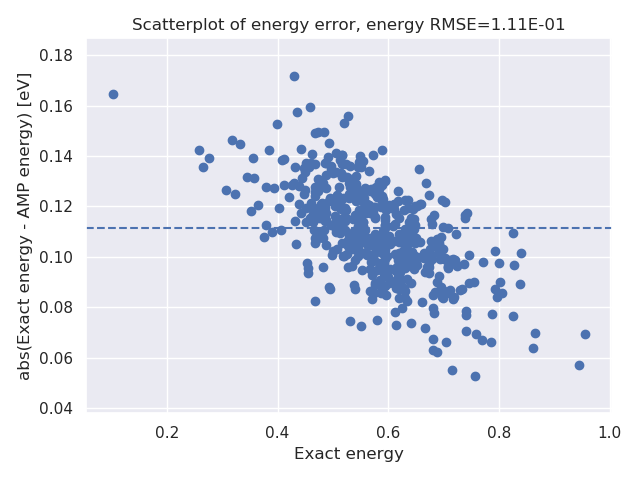
\includegraphics[width=\textwidth]{copper_energy_error.png}
      \caption{Energy error.}
    \label{fig:f1}
  \end{subfigure}
  \hfill
  \begin{subfigure}[b]{0.55\textwidth}
      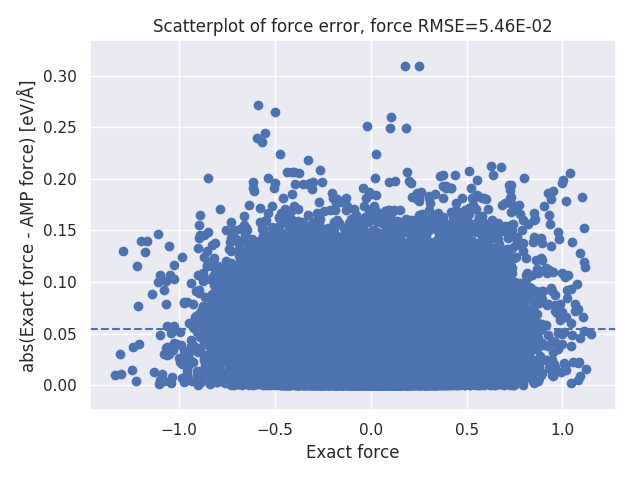
\includegraphics[width=\textwidth]{copper_force_error.png}
      \caption{Force component error.}
    \label{fig:f2}
  \end{subfigure}
\end{adjustbox}
    \caption{Energy and force component errors on test trajectory.}
    \label{fig:copper_error}
\end{figure}

In figure \ref{fig:copper_error} we have plotted the energy and force
absolute errors on the test images. We obtain an energy error
of approximately 0.1 eV, with a max value of approximately 0.16 eV.
For the force errors we obtain an force RMSE of 0.05 eV/Å,
but some of the force errors considerably higher, which poses
a problem for the long term stability of the system.

\begin{figure}[H]
    \centering
    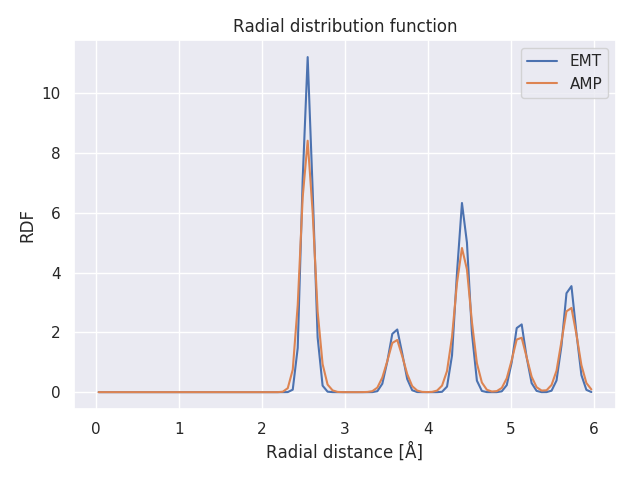
\includegraphics[width=\textwidth]{copper_rdf.png}
    \caption{AMP radial distribution function plotted against
        EMT RDF.}
    \label{fig:copper-rdf}
\end{figure}

In figure \ref{fig:copper-rdf} we have plotted the AMP neural network
radial distribution function compared to the EMT RDF.
We see that the AMP potential can reproduce the copper crystal
structure fairly well, though with smaller peaks.
The disparity is caused by an increase in kinetic energy over time
which makes the atoms more dispersed.

\begin{figure}[H]
    \centering
    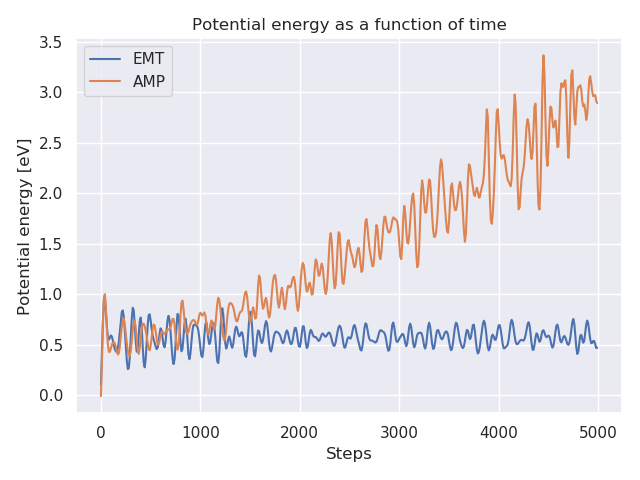
\includegraphics[width=\textwidth]{copper_pot.png}
    \caption{AMP and EMT potential energy as a function of time.}
    \label{fig:copper-pot}
\end{figure}

If we examine the potential energy as a function of time
in figure \ref{fig:copper-pot} we see that the neural network
follows the EMT potential energy fairly well for approximately
1500 steps, but then starts to significantly increase.
As the atoms are moved away from the potential
energy minimum the potential energy also starts to increase.
This is noticeable in figure \ref{fig:copper-energy},
where we have plotted the total energy as a function of time.
While the EMT energy is flat or oscillating around a mean value,
the neural network potential leads to increasing energy over time.
At the beginning the increase in energy appears to be attributable
to an increase in kinetic energy, which may be caused by errors
in the interpolated forces from the neural network.
This increase in kinetic energy also appears to lead to an increase
in translational momentum.

\begin{figure}[H]
    \centering
    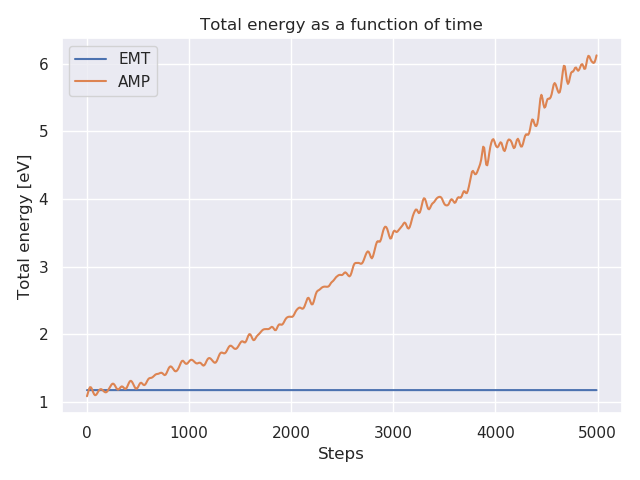
\includegraphics[width=\textwidth]{copper_energy.png}
    \caption{AMP and EMT total energy as a function of time.}
    \label{fig:copper-energy}
\end{figure}

\begin{figure}[H]
    \centering
    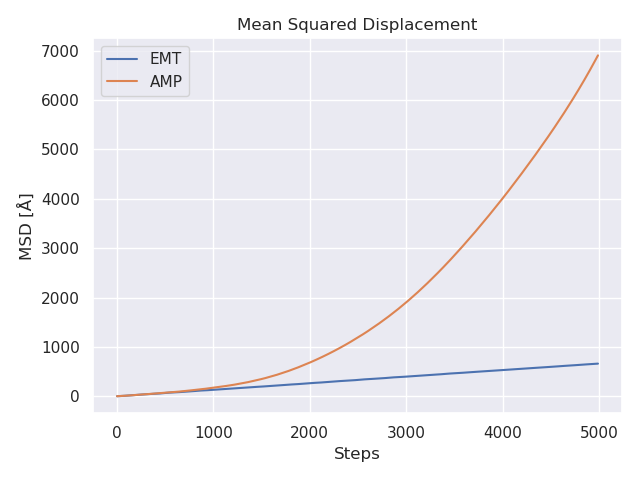
\includegraphics[width=\textwidth]{copper_msd.png}
    \caption{AMP and EMT mean squared displacements as a function of time.}
    \label{fig:copper-msd}
\end{figure}

In figure \ref{fig:copper-msd} we have plotted the mean squared
displacement, which is mean distance travelled averaged over all
atoms in the system.
We see that the MSD for the neural network is significantly larger
than for the EMT potential. In equilibrium we expect for a crystal lattice
that the mean squared displacement be linear, as the atoms
mostly oscillate in stable energy minimums and the motion can be
described by diffusion processes.
For the neural network potential the motion in the system appears
to be accelerating, as the kinetic and total energy is increased
over time.

\begin{figure}[H]
\begin{adjustbox}{max width=1.2\linewidth,center}
\centering
  \begin{subfigure}[b]{0.55\textwidth}
      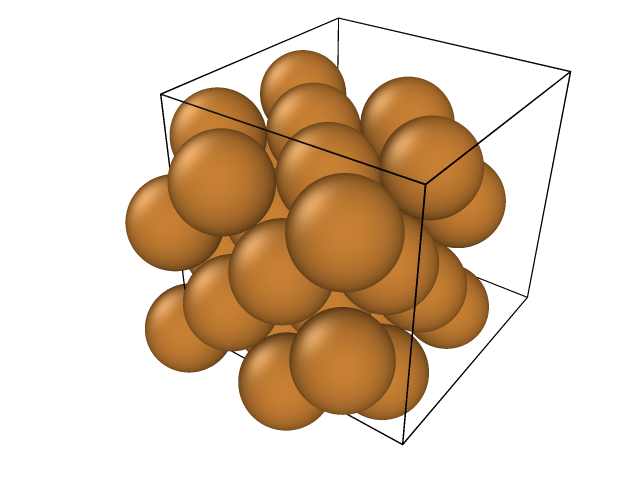
\includegraphics[width=\textwidth]{copper_t0.png}
      \caption{Copper atoms after 10 steps.}
    \label{fig:f1}
  \end{subfigure}
  \hfill
  \begin{subfigure}[b]{0.55\textwidth}
      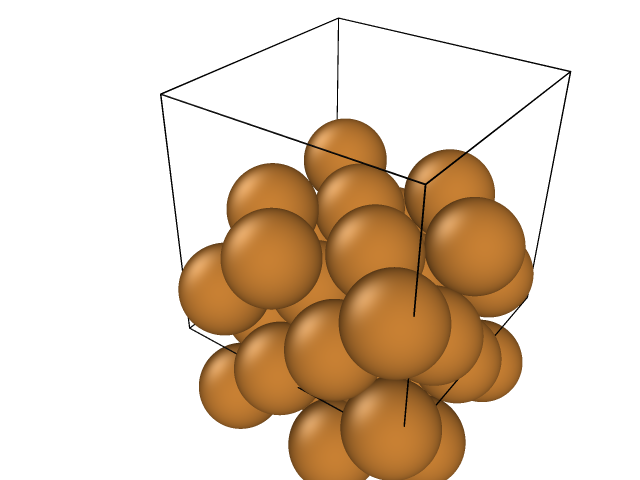
\includegraphics[width=\textwidth]{copper_tn.png}
      \caption{Copper atoms after 5000 steps.}
    \label{fig:f2}
  \end{subfigure}
\end{adjustbox}
    \caption{The system of copper atoms after 10 and 5000 steps.}
    \label{fig:copper_sw}
\end{figure}

If we examine the system trajectory in a program such as Ovito
\footnote{\href{Open VIsualization TOol}{https://www.ovito.org/}}
we find that the crystal structure has mostly remained intact, while the
system has picked up a certain amount of translational momentum.
In figure \ref{fig:copper_sw} we see that the system has moved as a whole,
although this is easier to see if you open up the trajectory file in Ovito
yourself.
This is in contrast to the EMT potential, in which the atoms vibrate in place
at this temperature, and the system remains more or less in place.
Altogether, this suggest that while the neural network potential
is able to reproduce the crystal structure, numerical errors propagate
to an increase in energy over time, which threatens the long-term numerical
stability of the trajectory. In order to obtain better results we would likely
require datasets containing more unlikely configurations and forces
(i.e. slightly out of equilibrium). We also generally find that the performance
improves as you add more symmetry functions, particularly radial functions
would improve the accuracy with this potential, as they are not explicitly
contained in the EMT potential. However, more symmetry functions
add significant CPU-time cost, and the set of symmetry functions would have to be pruned
to remove significant correlations.
Finally, we tested the time-scaling of the neural network as the number of atoms
increased. To test this we simply made a forces call on lattices of different
sizes which returns the force on every atom in the system.
Ideally we would have taken averages over multiple force calls, however
at this time scale we did not think it would significantly impact the results.

\begin{figure}
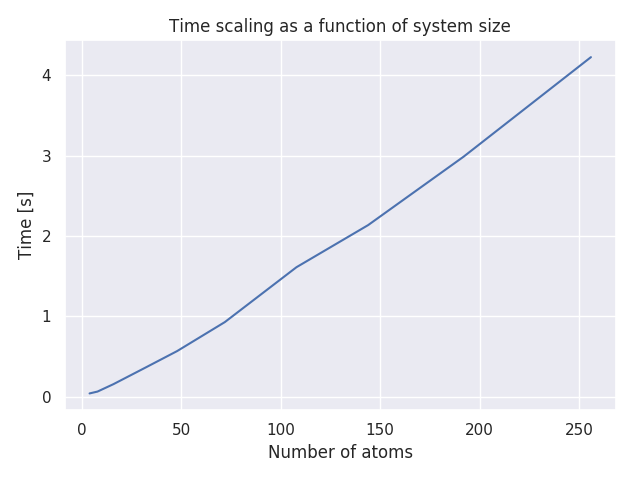
\includegraphics[width=\textwidth]{copper_scaling.png}
\caption{Time scaling of the neural network as size increases}
\label{fig:copper-scaling}
\end{figure}

In figure \ref{fig:copper-scaling} we see as expected that the trained neural network
scales linearly with the number of atoms, though with a significant pre-factor.
We see that it takes approximately 1 minute to evaluate all the forces
for a system of 60 atoms, while it takes 4 minutes for a system of 250 atoms.
This pre-factor is dependent on the average number of neighbors
of each atom, which is again dependent on the cutoff radius.
Since the neural network has been trained with a set cutoff radius,
this radius should deployed be considered a part of the neural network architecture
and cannot be significantly changed without impacting accuracy.
This pre-factor is of course also dependent on the time it takes to evaluate
the symmetry functions and derivatives, which is dependent on the number
and type of symmetry functions, as the angular function derivatives are significantly
more expensive to evaluate than the radial angular functions.
While linear scaling is desireable, the pre-factor is obviously too large,
as integrating a system of 250 atoms for 5000 steps would take almost 14 days!
However, this is only on a single core, and parallelizing using neighbor list algorithms
such as thouse found in the LAMMPS package could be a big improvement without too much overhead.
While this would help deployment, training would still be too slow.
As it stands now, the symmetry function derivatives have significant parts
implemented in Python which could with some effort be moved entirely to Fortran,
such as if-tests, dictionaries and neighbor lists.
If these parts of the codebase were moved fully to a lower-level compiled
language, this would help both training and deployment, and would enable
training and testing of larger and more complex systems.

\subsection{Stillinger-Weber}
The Stillinger-Weber is a potential which describes accurately
Silicon atoms in the diamond lattice structure, and was
one of the first potentials used to describe a realstic atomic-scale
model of Silicon. It is also one of the most common examples
of a potential with a threebody interaction, and its intermediate complexity
makes it ideal for verification with for example quantum calculations
or in our case machine learning methods.
As in the previous section we integrate the system over $8 \cdot 10^5$
steps using a timestep of $\Delta t = 5.0$ fs (suitable for most metals
in a crystalline structure) for a total of 8000 images for energy learning
and 500 images used to train forces. We train for 4000 epochs, since
the loss function is then usually suitably converged.
We generate a test set with identical positions and velocities
using the Stillinger-Weber potential and assess whether the neural network
can accurately reproduce the potential energy, radial distribution function
and more.

\begin{figure}[H]
\begin{adjustbox}{max width=1.2\linewidth,center}
\centering
  \begin{subfigure}[b]{0.55\textwidth}
      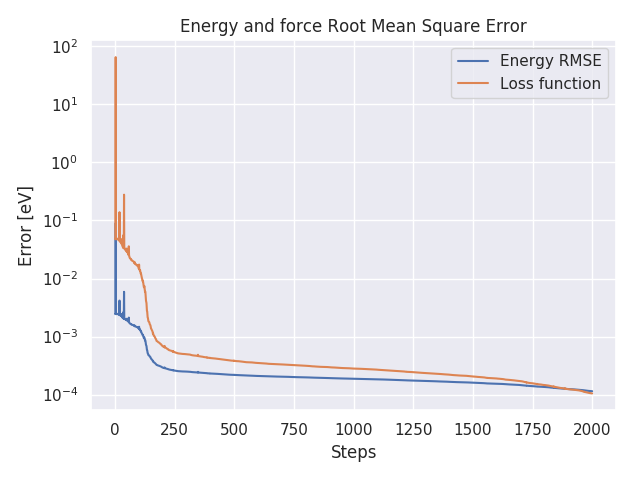
\includegraphics[width=\textwidth]{silicon_energy_log.png}
    \caption{Flower one.}
    \label{fig:f1}
  \end{subfigure}
  \hfill
  \begin{subfigure}[b]{0.55\textwidth}
      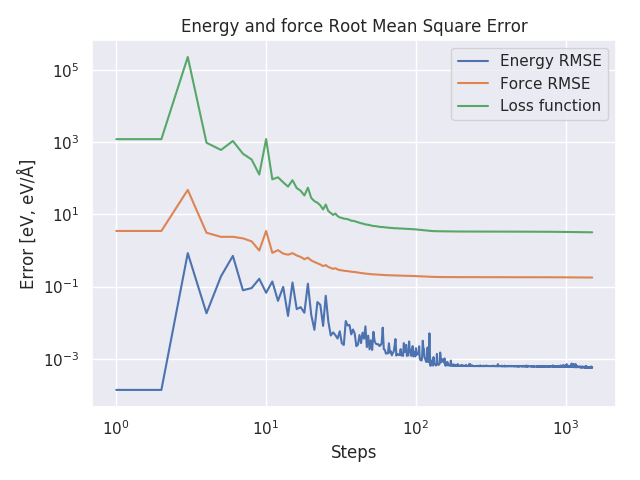
\includegraphics[width=\textwidth]{silicon_force_log.png}
    \caption{Flower two.}
    \label{fig:f2}
  \end{subfigure}
\end{adjustbox}
\caption{My flowers.}
    \label{fig:silicon-log}
\end{figure}

\begin{figure}[H]
\begin{adjustbox}{max width=1.2\linewidth,center}
\centering
  \begin{subfigure}[b]{0.55\textwidth}
      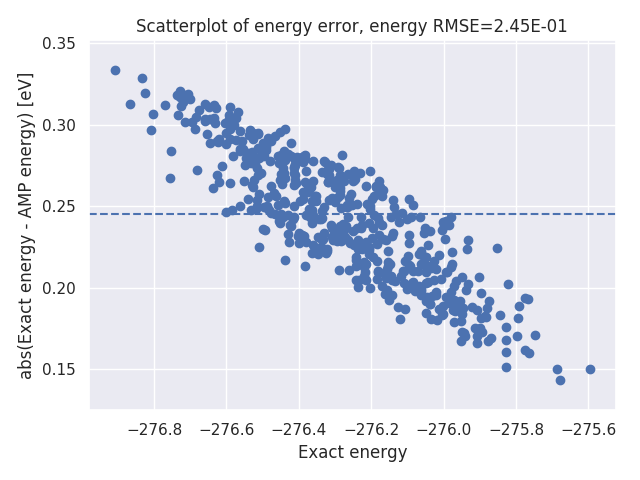
\includegraphics[width=\textwidth]{silicon_energy_error.png}
    \caption{Flower one.}
    \label{fig:f1}
  \end{subfigure}
  \hfill
  \begin{subfigure}[b]{0.55\textwidth}
      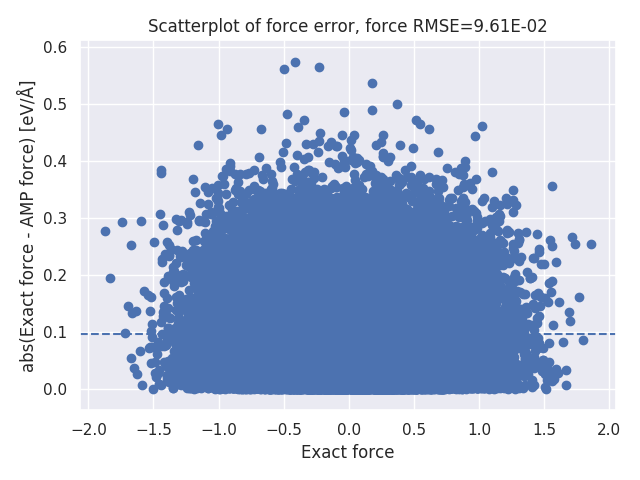
\includegraphics[width=\textwidth]{silicon_force_error.png}
    \caption{Flower two.}
    \label{fig:f2}
  \end{subfigure}
\end{adjustbox}
\caption{My flowers.}
    \label{fig:silicon-error}
\end{figure}

For the Stillinger-Weber trained neural network, we find that
the training errors for both the energies and forces are somewhat higher
in figure \ref{fig:silicon-log},
and this is also reflected in errors on the test set in figure \ref{fig:silicon-error}.


\begin{figure}[H]
    \centering
    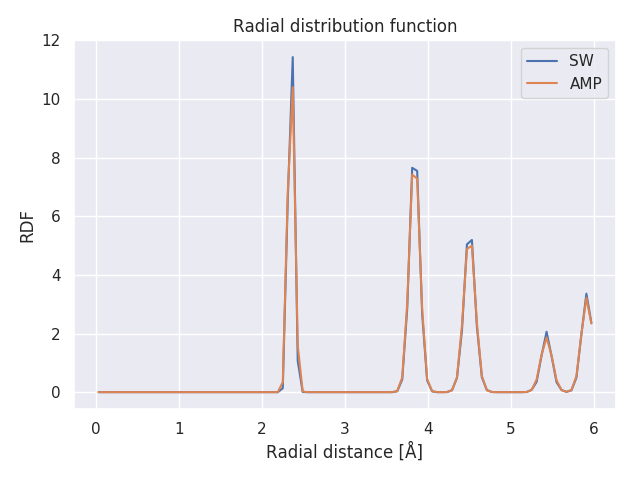
\includegraphics[width=\textwidth]{silicon_rdf.png}
    \caption{Caption}
    \label{fig:silicon-rdf}
\end{figure}

\begin{figure}[H]
    \centering
    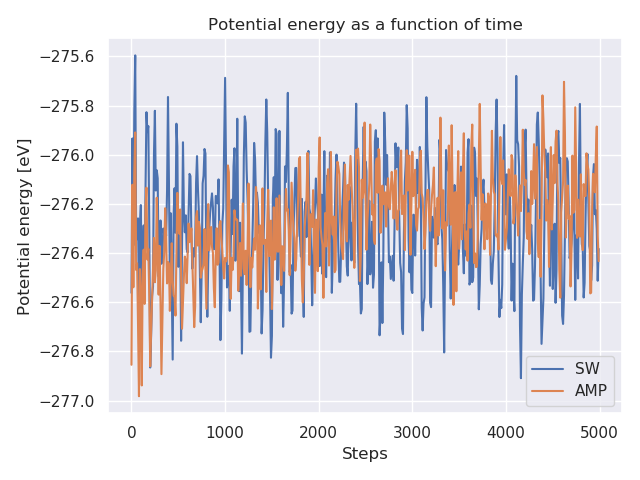
\includegraphics[width=\textwidth]{silicon_pot.png}
    \caption{Caption}
    \label{fig:silicon-energy}
\end{figure}

\begin{figure}[H]
    \centering
    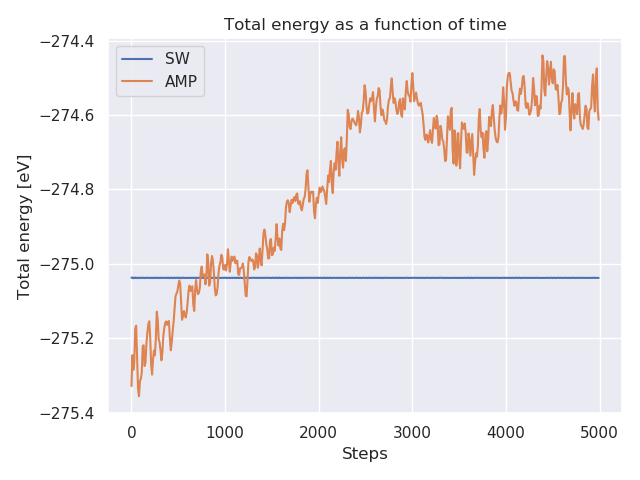
\includegraphics[width=\textwidth]{silicon_energy.png}
    \caption{Caption}
    \label{fig:silicon-energy}
\end{figure}

\begin{figure}[H]
    \centering
    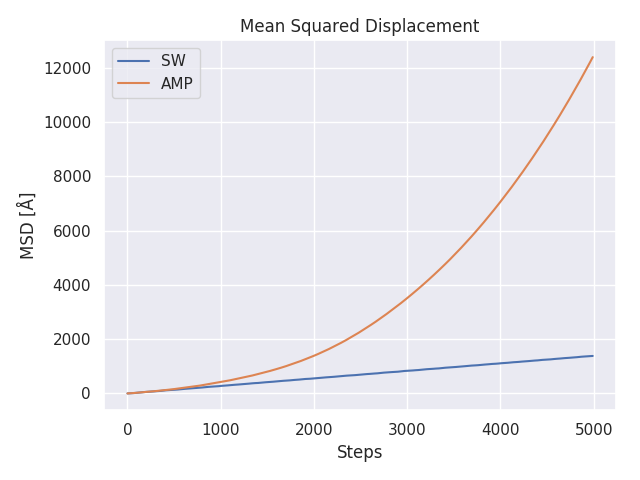
\includegraphics[width=\textwidth]{silicon_msd.png}
    \caption{Caption}
    \label{fig:silicon-energy}
\end{figure}
